\documentclass[review]{elsarticle}
% for submission use preprint
% review for

\usepackage{lineno,hyperref}
<<<<<<< Updated upstream
\usepackage{listings}
\usepackage{amsthm, amsmath,amssymb,amsbsy,amsfonts,amstext,rotating}
\usepackage{alltt,multicol,pifont}
\usepackage{booktabs,multirow,subfigure,epsfig}
\usepackage{xspace}
\newcommand{\eplopmark}{\ding{73}}
\usepackage{url}
\usepackage{tipa}
\usepackage{array,tabularx}
\usepackage{color}
\definecolor{applegreen}{rgb}{0.55, 0.71, 0.0}
\definecolor{bananayellow}{rgb}{1.0, 0.88, 0.21}
\definecolor{blue}{rgb}{0.0, 0.53, 0.74}
=======
\usepackage{amsmath}
\usepackage{xcolor}
>>>>>>> Stashed changes
\modulolinenumbers[5]

\journal{Journal of Networks and Computer Applications}

\renewcommand{\arraystretch}{0.7}

%%%%%%%%%%%%%%%%%%%%%%%
%% Elsevier bibliography styles
%%%%%%%%%%%%%%%%%%%%%%%
%% To change the style, put a % in front of the second line of the current style and
%% remove the % from the second line of the style you would like to use.
%%%%%%%%%%%%%%%%%%%%%%%

%% Numbered
%\bibliographystyle{model1-num-names}

%% Numbered without titles
%\bibliographystyle{model1a-num-names}

%% Harvard
%\bibliographystyle{model2-names.bst}\biboptions{authoryear}

%% Vancouver numbered
%\usepackage{numcompress}\bibliographystyle{model3-num-names}

%% Vancouver name/year
%\usepackage{numcompress}\bibliographystyle{model4-names}\biboptions{authoryear}

%% APA style
%\bibliographystyle{model5-names}\biboptions{authoryear}

%% AMA style
%\usepackage{numcompress}\bibliographystyle{model6-num-names}

%% `Elsevier LaTeX' style
\bibliographystyle{elsarticle-num}
%%%%%%%%%%%%%%%%%%%%%%%

\begin{document}

\begin{frontmatter}

\title{A wearable fall-detection system based on Body Area Networks for smart cities}

%% Group authors per affiliation:
\author{Luigi La Blunda\fnref{label1}}
\ead{l.lablunda@fb2.fra-uas.de (corresponding author)}
\author{Lorena Guti\'errez-Madro\~nal\fnref{label2}}
%% \author{Name\corref{cor1}\fnref{label2}}
\ead{lorena.gutierrez@uca.es}
\author{Matthias F. Wagner\fnref{label1}}
\ead{mfwagner@fb2.fra-uas.de}
\author{I. Medina-Bulo\fnref{label2}}
\ead{inmaculada.medina@uca.es}
\address[label1]{WSN and IOT Research Group Frankfurt University of Applied Sciences, Nibelungenplatz 1, 60318 Frankfurt am Main, Germany}
\address[label2]{UCASE Software Engineering Research group, University of Cadiz}



%% or include affiliations in footnotes:
%\author[mymainaddress,mysecondaryaddress]{Elsevier Inc}
%\ead[url]{www.elsevier.com}
%
%\author[mysecondaryaddress]{Global Customer Service\corref{mycorrespondingauthor}}
%\cortext[mycorrespondingauthor]{Corresponding author}
%\ead{support@elsevier.com}
%
%\address[mymainaddress]{1600 John F Kennedy Boulevard, Philadelphia}
%\address[mysecondaryaddress]{360 Park Avenue South, New York}

\begin{abstract}
Falls can have serious consequences for people, which can lead, for example, to restrictions in mobility or in the worst case to traumatic based cases of death. To provide rapid assistance, a portable fall detection system has been developed which is capable of detecting fall situations and, if necessary, alerting the emergency services without any user interaction. The prototype was designed to facilitate a reliable fall-detection and to classify several fall-types. This solution represents a life-saving service for every inhabitant which would significantly enrich the development of smart cities and smart factories where fall-events are part of daily-life. This paper will also introduce the fall analysis, which includes the generation of test events. To guarantee functional safety, the hazard analysis method STAMP (System-Theroetic Accident Model and Processes) will be applied. 
\end{abstract}

\begin{keyword}
e-Health \sep fall-detection\sep Body Area Network \sep safety \sep STAMP \sep Smart City \ 
\end{keyword}

\end{frontmatter}

%\linenumbers

\section{Introduction}
Fall-detection is gaining in importance not only in aging societies, but also in the working society and in daily activities. According to the World Health Organization (WHO), 646,000 fatal falls are estimated to be the second leading cause of accidental or unintentional death worldwide each year. People over 65 suffer the most fatal falls. Another high risk group is children. Taking into consideration their evolving developmental stages, the increasing curiosity to explore the environment or the inadequate adult supervision lead to fall-events \cite{WHO2018}.
In everyday life we are also confronted with risk of falling. Working in hazardous working conditions is another risk factor for causing fall-events. An exemplary event could be a worker who falls during the night shift in the factory and no one is there to provide prompt assistance. Another example could be a technician which falls from height while maintaining windmills. Mostly windmills are installed in uninhabited areas where no immediate rescue measures can be taken. Considering these events the consequences can be fatal for the affected people. 
The World Health Organization stated that annually 37.3 million fall-events are severe enough to require medical treatment \cite{WHO2018}. Fall-events leads to the side effects of physical inactivity and loss of balance, especially among old people. Elderly people are scared to fall again and this uncertainty of movement increases the risk of repeated falls. 
To counteract these life-threatening events fast assistance is necessary due to the fact that an unconscious person may not be able to call the emergency services. An approach could be the continuous tracing of medical and / or physical parameters via a wearable sensor network (see Figure \ref{fig:escalationscheme}).
\begin{figure}[!ht]
	\centering
	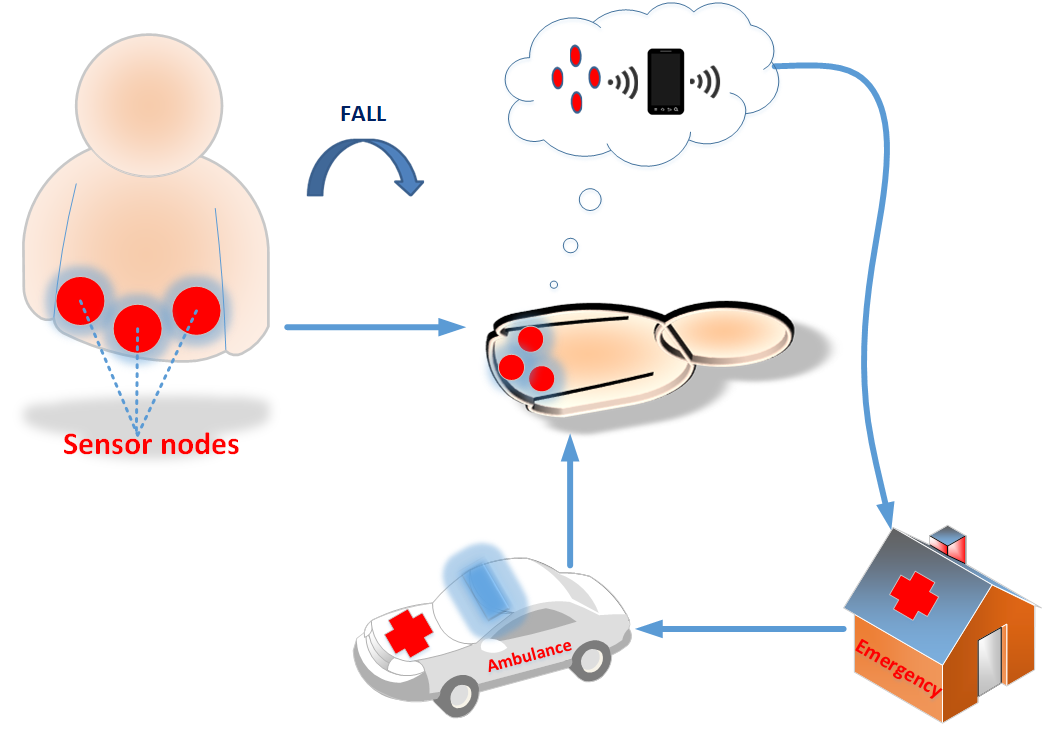
\includegraphics[scale=0.35]{Images/EscalationScheme}
	\caption[Escalation scheme]{Escalation scheme simulation~\cite{LaBlunda.2016,LaBlunda.2016b}}
	\label{fig:escalationscheme}
\end{figure}
A prototype in form of a belt was developed which includes an Electrocardiogram (ECG) - harness and is based on a five sensor nodes Body Area Network (BAN). Each sensor node of the belt acquires continuously acceleration data including time stamp and the sensor node of the ECG-harness provides the analog value of the voltage including time stamp. In case of a fall the system should be capable to autonomously call the emergency services. Applying sensor fusion of physical and medical sensors we expect to improve the reliability of fall-detection and possibly fall-prevention. Another expectation is that the integration of medical sensors may facilitate the classification of different fall-types. In terms of smart cities our expectancy is to significantly provide an important e-health service for smart cities which is an essential life-saver for the population.

The paper is structured as follows. Section \ref{sec:relatedwork} describes the related work regarding fall-detection. In this section a short overview about existing solutions and different approaches for fall-detection is given. Section \ref{sec:background} will describe the basic principles on which our ongoing fall-detection research is based. In the successive section (Section \ref{sec:fall-detectionPrototype}) a detailed description of the fall-detection prototype, including the usage of the ECG-sensor are introduced. Additionally, this section contains the generation of test events which includes the results of the fall-analysis and detected problems. Section \ref{sec:STAMP} will introduce the Hazard analysis method STAMP \cite{leveson2011engineering} which is applied on the fall-detection prototype.
Finally, in section \ref{sec:conclusion} a conclusion about this ongoing research is given, including some indications for improvement which could be applied in the future work.

\section{Related Work}
\label{sec:relatedwork}
In this section an overview about several fall-detection approaches is given. There are several techniques which can be applied to detect fall-events. Igual et al. \cite{Igual2013} illustrates the following different types of fall-detection  systems:
\begin{itemize}
	\item Context-aware systems
	\item Wearable systems
\end{itemize}
The functionality of context-aware systems depends on the environment, since the sensors and actuators must be installed in the living area (apartment, nursing home) in order to detect possible fall situations. The video-based context-aware solutions have the advantage to provide an accurate and reliable detection of falls with a fast assistance, but these systems have an issue regarding privacy. Patients using this solution are non-stop monitored and this is not well accepted by many. Additionally, the high purchase price is an obstacle for many patients and the dependency on the environment makes this approach useless in many application scenarios, because it would not detect fall-events happening outside the networked area.

The other category of fall-detection systems analyzed by Igual et al. \cite{Igual2013} contains wearable solutions worn on the body and are based on Body Area Networks (BAN). This solution is capable to provide a fall-detection which is independent from the environment in contrast to context-aware systems. The analysis of Igual et al. \cite{Igual2013} illustrates wearable fall-detection systems using the sensor fusion method which comprises accelerometer and gyroscope data and built-in systems in form of smart phone sensors. For both categories of fall-detection solutions (context-aware \& wearable solution) several techniques were used. The following methods were applied for context-aware systems:
\begin{itemize}
	\item Image processing and threshold-based recognition
	\item Image processing and classification models
\end{itemize}
The techniques used for the fall-detection in wearable solutions are the following:
\begin{itemize}
	\item Threshold-based approach
	\item Fall-detection based on machine learning based data analysis
\end{itemize}
Taking into consideration the fact that it is an essential advantage to focus on wearable solution because of the system's functional independence the scientific work of Li et al. \cite{Li2009} will be explained subsequently. The solution of Li et al. \cite{Li2009} includes two wearable sensor nodes which are based on a BAN. These sensor nodes consist of an accelerometer and gyroscope and they are placed on the chest (Node A) and on the thigh (Node B, see Figure \ref{fig:LietAl-Architecture}). 
\begin{figure}[!ht]
	\centering
	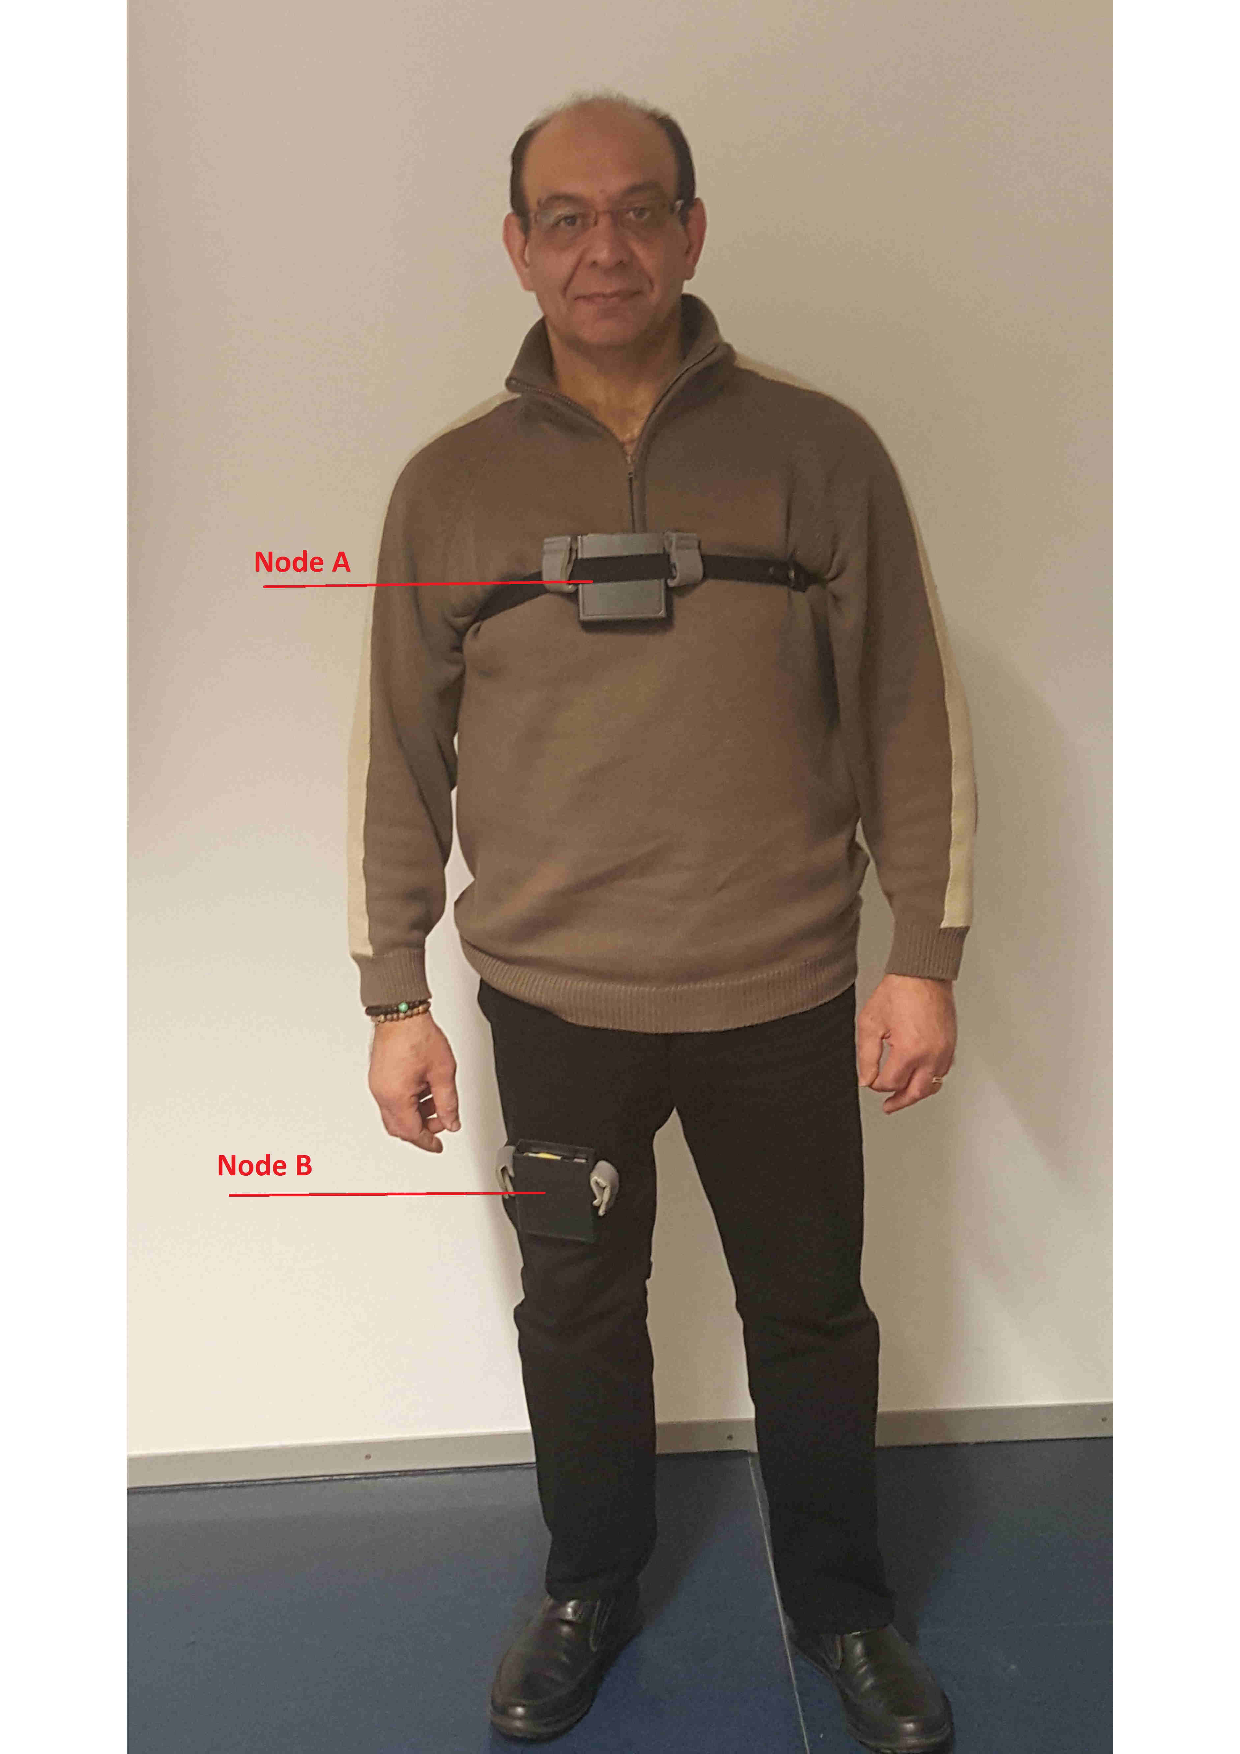
\includegraphics[scale=0.375]{Images/Stankovic-papa2.pdf}
	\caption[System architecture according to Li et al.]{System architecture according to Li et al. \cite{Li2009}}
	\label{fig:LietAl-Architecture}
\end{figure}
Li et al. distinguish between two different motion sequences which are used for activity categorization:
\begin{itemize}
	\item Static postures:
	\begin{itemize}
		\item Standing, sitting, lying
	\end{itemize}
	\item Dynamic postures:
	\begin{itemize}
		\item Activities of daily life (ADL) $\rightarrow$ walking, go up / down stairs, sit, jump, lay down, run
		\item Fall-like motions $\rightarrow$ quick sit-down upright, quick sit-down reclined
		\item Flat surface falls $\rightarrow$ fall forward, fall backward, fall right, fall left
		\item Inclined falls $\rightarrow$ fall on stairs
	\end{itemize}
\end{itemize}
A 3-phase algorithm for fall-detection is proposed by Li et al. \cite{Li2009} to decrease the computational effort of the micro controller. The first phase of the fall-detection algorithm examines if the person is in a static or dynamic position. If the analyzed position coincides with a static postures in the second phase it will be checked whether it corresponds to lying. If in lying position, it will be checked if the transition to this posture was intentional or unintentional (3 \textsuperscript{rd} phase). To determine it, the previous 5 seconds of data is used. In the case it was unintentional the event will be classified as a fall. The proposed approach in \cite{Li2009} uses a threshold based technique that is applied in the different phases of the algorithm. The weakness of this approach is to differentiate between jumping into bed and falling against wall with seated posture. Collado Villaverde et al. \cite{colladomachine} propose a wearable fall-detection solution based on a smartwatch using acceleration data in combination with machine learning techniques.

A different approach to detect fall-events is presented by Lüder et al. \cite{Luder2009} which apply an air pressure sensor in addition to the accelerometer. The minor air pressure changes correspond to an altitude change of 25 cm which is a relevant indication in combination with accelerometer data of a possible fall-event.  This sensor combination is incorporated in the hardware "StairMaster" of the Frauenhofer Institute. The hardware architecture proposed in \cite{Luder2009} depicts a wearable solution which is worn on the hip and provides wireless data transmission via Bluetooth. Alternatively, the data can be stored on a Secure Digital (SD) card for evaluation purposes. Due to the fact that air pressure can be influenced by meteorological disturbances Lüder et al. \cite{Luder2009} introduced an alternative architecture. This alternative approach incorporates an external barometric sensor as a reference, which is placed in a stationary altitude to compare both air pressure data (wearable \& stationary). Another method for fall-detection based on sensor fusion techniques is described by Gjoreski et al. \cite{Gjoreski2014}. Accelerometer and electrocardiogram (ECG) data is used to detect fall-events. The solution in \cite{Gjoreski2014} is capable of identifying person's movements and fall-situations using wearable sensor nodes based on Bluetooth. These nodes are placed on the chest and thigh which is similar to Li et al's \cite{Li2009} approach. The advantage of the proposed solution by Gjoreski et al. \cite{Gjoreski2014} is the integration of medical sensors. The fusion of acceleration data and ECG-Signal facilitates the detection of anomalies in person's behavior and heart related problems that my lead to falls. The results presented in \cite{Gjoreski2014} emphasize that the incorporation of the ECG-signal can significantly increase the system's reliability to detect fall-events. According to the analysis of Gjoreski et al. \cite{Gjoreski2014} differences in the ECG-signal in different postures were detected. Lower beat rates in the static positions lying and sitting compared to waling were determined. Comparing the beat rates of both static postures (lying and sitting) differences were observed, where the beat rate of lying is lower than the one of sitting.



\section{Background}
\label{sec:background}
The fall-detection prototype is based on the approach proposed in \cite{Gjoreski2014, Kozina}. To detect a fall-event a typical physical behavior is used which comprises the following the phases (see Figure \ref{fig:fallKozina}):
\begin{itemize}
	\item Pre-fall-phase 
	\item Falling phase
	\item Impact phase
	\item Post-fall phase
\end{itemize}
The pre-fall phase illustrates a stationary position of the person where the measured acceleration is around 1g (9.81$m/s^{2}$). During the falling phase the  acceleration decreases close to 0g (0$m/s^{2}$), which depicts a similar behavior to a free fall. Upon the impact (impact phase), the acceleration reaches his maximum value for a short period of time. This signalizes that the person has suffered an impact. Subsequently, the acceleration is decreasing to around 1g (9.81$m/s^{2}$) which represents the post-fall phase because after a fall the person is lying down. To apply this fall-detection pattern the accelerometer data of the sensor nodes is used. Important to know is that for the impact detection the acceleration magnitude is used which is calculated with the following formula ~\ref{eq:acel} and to determine the body's orientation the single axis values of the accelerometer ($\alpha_x$, $\alpha_y$, $\alpha_z$) are analyzed:

\begin{equation}\label{eq:acel}
\alpha = \sqrt{\alpha_{x}^{2} + \alpha_{y}^{2} + \alpha_{z}^{2}}
\end{equation}

\begin{figure}[!ht]
	\centering
	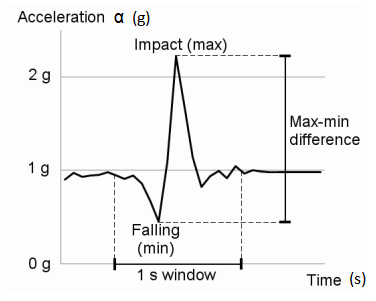
\includegraphics[scale=1]{Images/KozinaImpact}
	\caption[Acceleration during impact]{Acceleration during impact according to Kozina et al. ~\cite{Kozina}}
	\label{fig:fallKozina}
\end{figure}
Taking into consideration the body orientation the single acceleration axis ($\alpha_x$, $\alpha_y$, $\alpha_z$) are essential to determine the person's body orientation. Assuming that the person is in a standing position (static posture), the x-acceleration ($\alpha_x$) corresponds to 1g (9.81$m/s^{2}$) and the other two axis ($\alpha_y$, $\alpha_z$) would be close to 0g (0$m/s^{2}$). As soon as the person changes his posture, the gravitational force will act on one of the other two axis ($\alpha_y$, $\alpha_z$) and the x-acceleration will be 0g (0$m/s^{2}$). Combining this information with the acceleration magnitude (see Equation \ref{eq:acel}) the system is able to detect the fall and additionally determine the type of fall.

To ensure reliable fall detection, the system must be able to detect various types of falls. For this reason, the development of the fall detection prototype is also based on the creation of a test protocol covering different types of falls. The scientific papers by Li et al. \cite{Li2009} and Pannurat et al. \cite{Pannurat2014} were chosen as a reference, as they not only represent possible solutions for fall detection, but also offer a versatile overview of possible fall scenarios.

\section{Fall-detection system prototype}
\label{sec:fall-detectionPrototype}	

\subsection{Architecture}
\label{subsec:Architecture}	
The hardware architecture plays an important role in the development process to ensure the reliable functioning of the system. A first prototype was developed in this ongoing research which is introduced in \cite{LaBlunda.2016, LaBlunda.2016b}. This paper presents an improved version of the prototype in \cite{LaBlunda.2016, LaBlunda.2016b}, which includes essential developments that contribute to reliable operation of the system. Additionally, the improved hardware design meets the requirement for patient compliance. This aspect should be taken into consideration to provide a user friendly design which facilitates the freedom of movement for the user. As a safety critical system for medical purposes, a redundant hardware design should be provided to protect the system against a total system failure which would have severe consequences for the user in case of fall-events. Referring to J{\"a}ms{\"a} et al. \cite{jamsa2014fall} the best approach is to position the accelerometer near to the waist. Taking into consideration these aspects a wearable belt solution was developed which is based on a four sensor nodes BAN (see Figure \ref{fig:BanBelt}).
\begin{figure}[!ht]
	\centering
	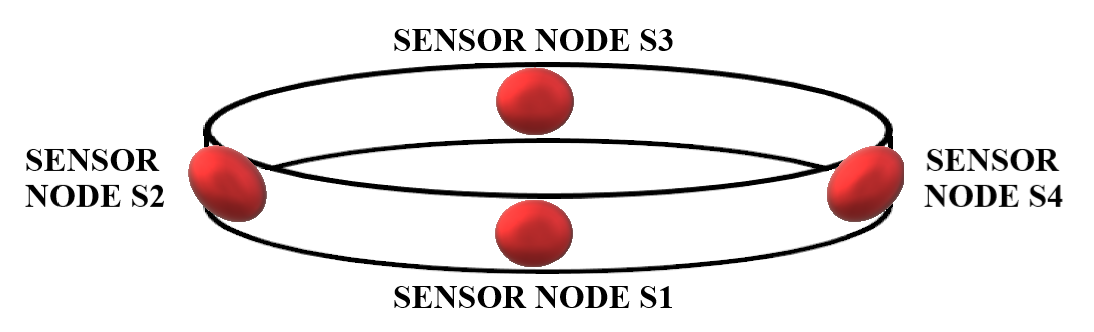
\includegraphics[scale=0.41]{Images/belt}
	\caption[Four sensor nodes BAN - Belt]{Four sensor nodes BAN - Belt \cite{LaBlunda.2016, LaBlunda.2016b}}
	\label{fig:BanBelt}
\end{figure}

The four sensor nodes (S1 - S4) positioned on the belt are acting as peripherals and are continuously acquiring acceleration data which is sent via Bluetooth Low Energy to the smart phone (central device). The dataset consists of the following information: 
\begin{center}
 SensorID, X-Acceleration, Y-Acceleration, Z-Acceleration
\end{center}
\begin{itemize}
	\item \textbf{SensorID} $\rightarrow$ is used to identify to which sensor node the incoming dataset belongs to.
	\item \textbf{X-Acceleration} $\rightarrow$ represents the acceleration value $\alpha_{x}$ in X-direction which includes the unit m/$s^2$.
	\item \textbf{Y-Acceleration} $\rightarrow$ represents the acceleration value $\alpha_{y}$ in Y-direction which includes the unit m/$s^2$.
	\item \textbf{Z-Acceleration} $\rightarrow$ represents the acceleration value $\alpha_{z}$ in Z-direction which includes the unit m/$s^2$.
\end{itemize}
The central device receives the incoming sensor data which will be stored in separate data files to evaluate the event. 
The belt solution reflects the above criteria of a safety-critical systems. The proposed architecture (see Figure \ref{fig:BanBelt}) is based on a mirroring principle of the opposite sensor nodes which provide identical acceleration values, only with different signs. If a sensor node fails during operation, the opposite node can be used as a reference to ensure accurate evaluation of the event.  Considering the following scheme (see Figure \ref{fig:ReferenceScheme}) this fall-detection belt solution facilitates the recognition of different fall-event types. 

\begin{figure}[!ht]
	\centering
<<<<<<< Updated upstream
	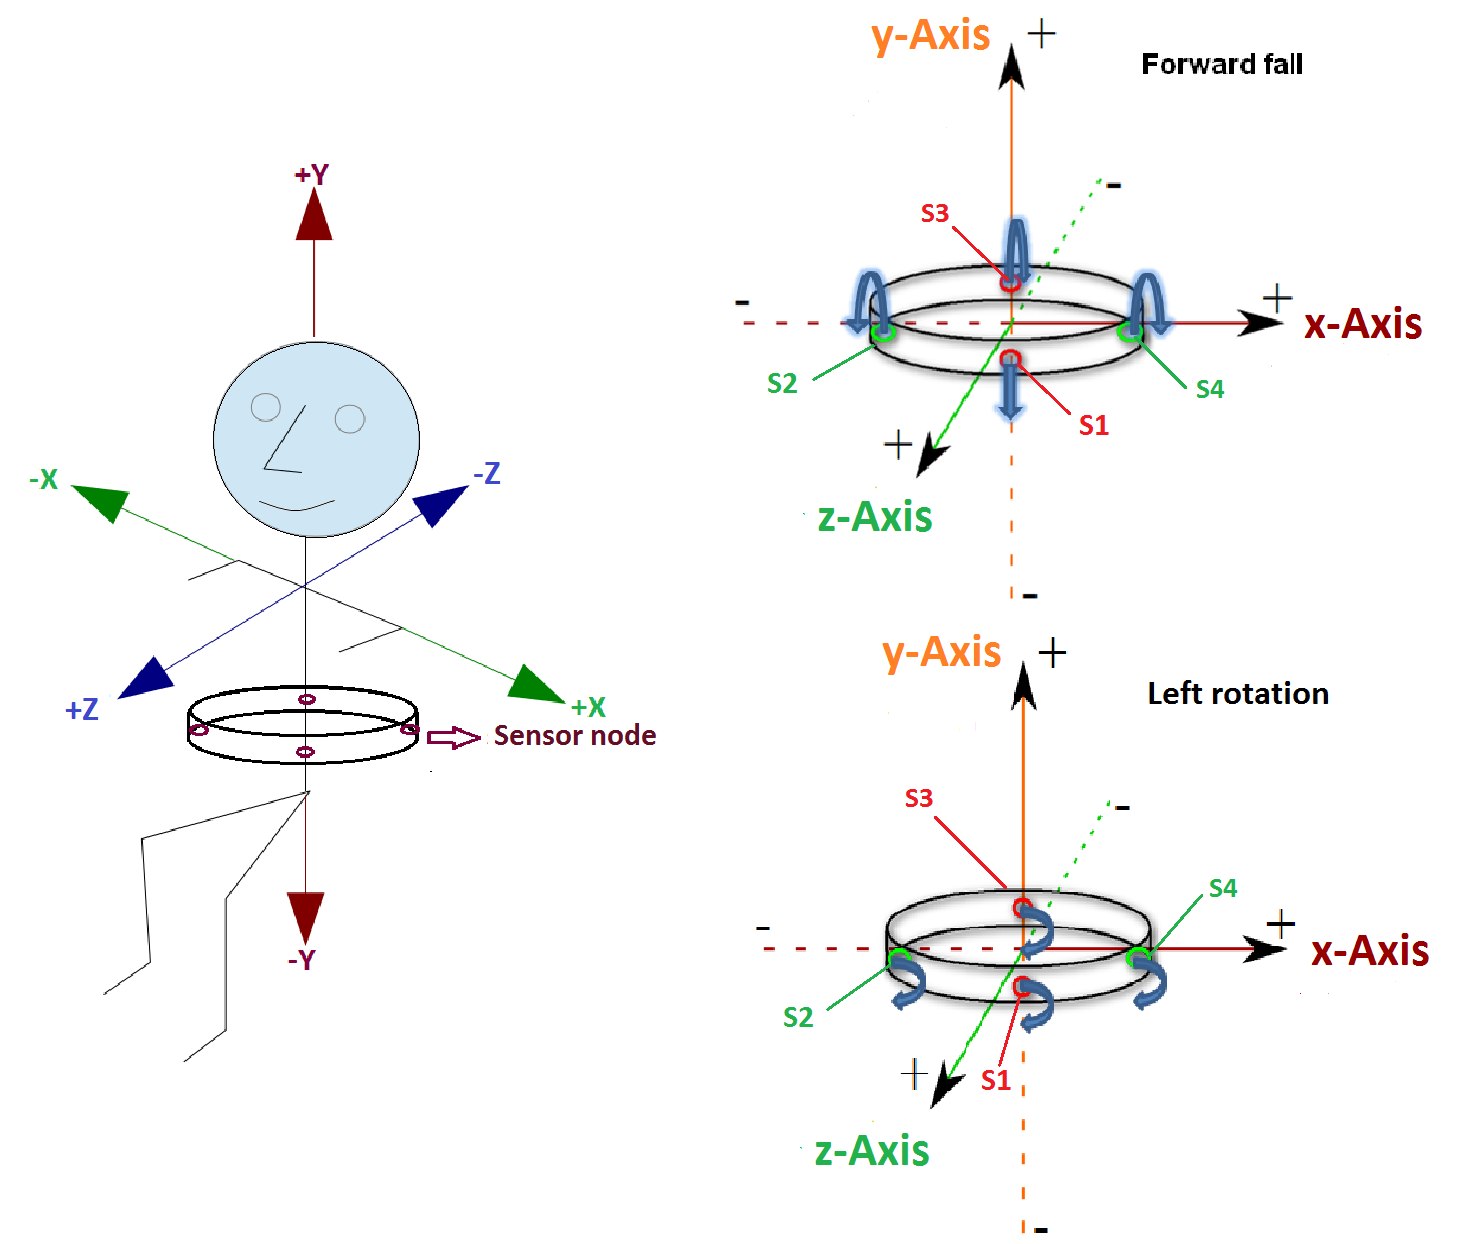
\includegraphics[scale=0.28]{Images/axis}
=======
	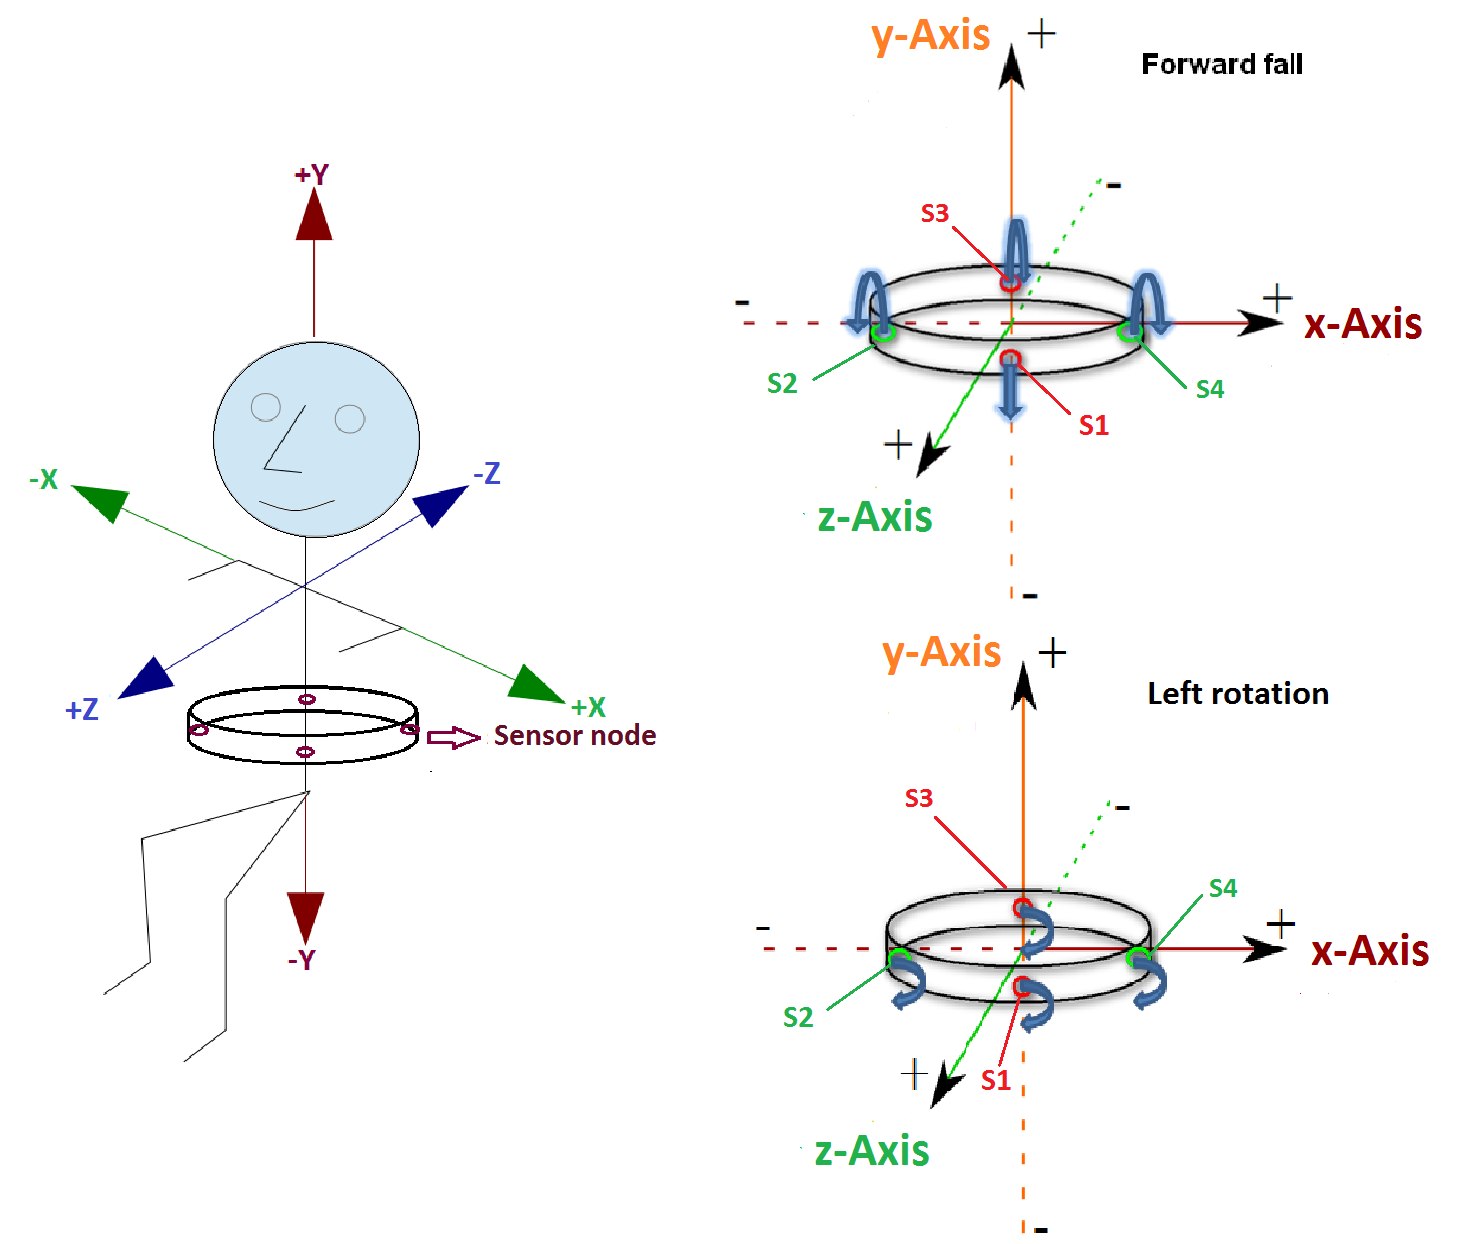
\includegraphics[scale=0.29]{images/axis}
>>>>>>> Stashed changes
	\caption[Three axis reference scheme]{Three axis reference scheme \cite{LaBlunda.2016,LuigiMasterThesis}}
	\label{fig:ReferenceScheme}
\end{figure}
The positioning of the nodes around the hip allows a precise fall-characterization.
As an example, a person is taken who has suffered a frontal fall because of a fainting. Analyzing the fall-event, it can be determined that the fall caused by a fainting leads firstly to a left rotation of the person's body (pre-fall phase). This event triggers the fall of the person (impact to the ground). Projecting this fall event on the reference scheme (see Figure \ref{fig:ReferenceScheme}), the body's orientation (e.g. left rotation) can be determined on the basis of the individual acceleration values ($\alpha_x$,  $\alpha_y$,  $\alpha_z$). Additionally, the acceleration magnitude (see Equation \ref{eq:acel}) can be used for the detection of the impact which is categorized by a temporary increase in the acceleration, as described in the previous section \ref{sec:background}.
Taking into consideration the test protocol stated in section \ref{sec:background} typical fall-events (e.g. rolling out of the bed) in nursing homes and hospitals can be detected by this solution.


\subsection{Sensor fusion}
\label{subsec:sensorfusion}	
Analyzing the literature regarding fall detection, it was pointed out that the existing solutions show certain weaknesses in the reliable detection of falls \cite{Igual2013, Li2009, Luder2009, Pannurat2014, jamsa2014fall}. Considering Gjoreski et al. approach, his results with the fusion of physical sensors and the ECG sensor show a reliable fall detection. Especially the evaluation of the ECG signal leads to an essential improvement of the system's accuracy.  According to \cite{Gjoreski2014} the ECG signal could be used to distinguish between different postures. The inclusion of medical parameters could even provide a fall prediction that would represent a significant progress in health care and prevent fatal injuries. Based on these results the proposed fall-detection belt  has been upgraded with a portable 3-channel ECG-sensor which provides an analog signal to the microcontroller. The successive illustration depicts the BAN structure of the update prototype architecture.
\begin{figure}[!ht]
	\centering
	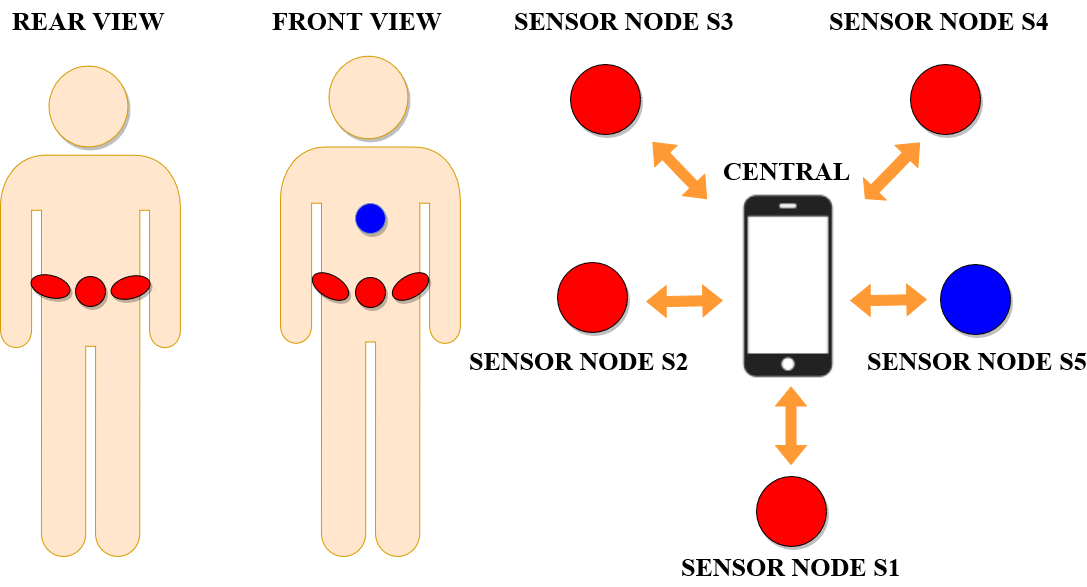
\includegraphics[scale=0.27]{Images/ECG-BAN.png}
	\caption[ECG - BAN]{ECG - BAN}
	\label{fig:ECGBAN}
\end{figure}
The updated BAN includes four sensor nodes placed on the belt (S1 - S4) and an additional node on the chest (S5). These five nodes are acting as peripherals and they are continuously providing sensor data to the smart phone (central) via Bluetooth Low Energy. The sensor nodes S1 to S4 send the acceleration data and the ECG-sensor sends analog values (representation of ECG-signal) to the central device. Fusing these information the central device analyzes the events for possible fall-events.

Before the ECG-sensor can be fully integrated into the prototype, some tasks had be solved.  The first task to solve is a continuous recording of the ECG during the person's daily activities. The first task will be to facilitate a stable and continuous recording of the ECG, even during the person's daily activities. When the ECG-electrodes lose contact with the skin surface because of movement, this leads to increased noise in the signal. Therefore, a solution for reliable ECG-recording have to be developed. The second task is to perform a validation of the ECG-sensor. For this purpose, the own ECG-measurements must be compared with measurements taken by a medically certified clinical ECG-device, in order to guarantee the correctness of the ECG-values. Based on Gjoreski et al. \cite{Gjoreski2014} the ECG-signal is relevant to detect fall-events as mentioned in section \ref{sec:relatedwork}. Based on this, another task will be the determination of ECG patterns that provide relevant information for fall events.

The first test measurements with the ECG sensor confirmed the noisy and unstable ECG signal during movements. To ensure a stable and continuous signal during daily activities, an adjustable and flexible ECG-harness has been developed with prefabricated electrodes positioning and the ability to adapt to any body shape (see Figure \ref{fig:ECGHarness}).
\begin{figure}[!ht]
	\centering
	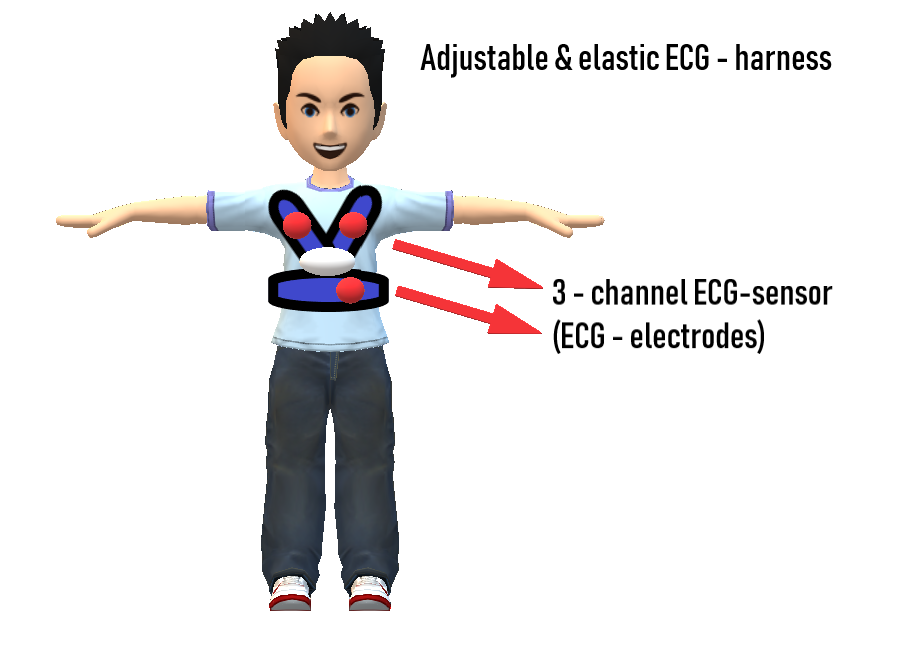
\includegraphics[scale=0.35]{Images/ECG-Harness.png}
	\caption[ECG - Harness]{ECG - Harness}
	\label{fig:ECGHarness}
\end{figure}
After completing the development of the ECG-harness the measurements were repeated using the harness solution. A more stable signal resulted, especially during walking and the sitting procedure the stability of the ECG-signal was improved significantly. The artifacts in an ECG-signal which result during motion may be used as a recognition pattern for fall-events. After the positive results regarding the improvements of the signal's stability, validation tests were conducted in a medical lab with the assistance of a physician. In clinical settings ECG-devices with 10 electrodes are being used but for wearable or emergency purposes (e.g. ambulance) a 3-Channel ECG-device is recommended because it provides less wiring and satisfies the aspect of patient compliance \cite{DrNicoletteWagner}. According to a study by Antonicelli et al. \cite{Antonicelli-ECG}, the use of a 3-lead ECG may be essential to avoid delayed treatment of specific heart diseases, such as elderly people who suffer from chronic heart disease and need continuous ECG monitoring. In addition, the analysis in \cite{Antonicelli-ECG} led to the result that a 3-lead ECG provides qualitatively similar evaluation as a 12-lead ECG.    Comparing the measurements taken in the medical lab with the ECG-measurements provided by our ECG-sensor the correct functionality of our sensor could be confirmed. The used sensor architecture only differs in signal quality that includes noise and baseline shifting. The reasons for these distinctions in signal quality were explained by the supervising physician. Baseline wander (BW) disturbances are caused by variations in electrode-skin impedance, patient's movement and breathing during the ECG-measurements. Considering amyostasia disturbances the ECG-signal is affected by contraction of muscles near the heart which lead to additional noise in the signal. Muscle contraction is common for people which suffer from tremor or fearing the ECG-measurement and for disabled people. The certified medical devices have an integrated filter which can be applied, to smooth the signal \cite{ECGNoise,DrNicoletteWagner}. 

\subsection{Generation of test-events}

\subsection{IoT test event generator}
\label{iotteg}

IoT-TEG~\cite{TesisGutierrez2017,Gutierrez2017} is a Java-based tool which takes an event 
type definition file and a desired output format (JSON, CSV, and XML, the most common across 
IoT platforms). IoT-TEG is made up of a \emph{validator} and an \emph{event generator} 
(Figure~\ref{fig:IoT-EGArquitecture}). The validator ensures the definition follows the rules set 
by IoT-TEG. The generator takes the definition and generates the indicated number of events according to it.

\begin{figure}[!ht]
  \centering
  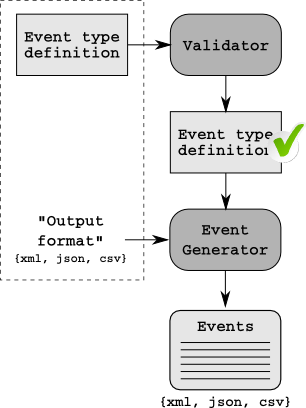
\includegraphics[scale=0.65]{Images/IoT-EGArquitecture}
  \caption[IoT-TEG Architecture]{IoT-TEG Architecture~\cite{TesisGutierrez2017,Gutierrez2017}.}
  \label{fig:IoT-EGArquitecture}
\end{figure}

Previous studies suggested there were no differences in testing effectiveness between using events
generated by IoT-TEG, or events recorded from various case studies~\cite{TesisGutierrez2017,Gutierrez2017}.
Moreover, thanks to its implementation, IoT-TEG can be used to do different type of test: functional,
negative, integration, stress, etc; in deed an example of its usability can be found 
in~\cite{TesisGutierrez2017,gutierrez2018}, where IoT-TEG has been used to apply the mutation 
testing~\cite{jia2011}. These results confirm IoT-TEG can 
simulate many types of events occurring in any type of applications, it can do different type of tests
and it can solve the main challenges developers face when they test event-processing programs:
\begin{enumerate}
 \item Lack of data for testing,
 \item needing specific values for the events, and
 \item needing the source to generate the events.
\end{enumerate}

For the sake of clarity, Example~\ref{eventTypeDef} shows an event type
definition.

\begin{lstlisting}[basicstyle=\ttfamily\footnotesize,language=XML,caption=Event type definition example,label=eventTypeDef]
<?xml version="1.0" encoding="UTF-8"?>
<event_type name="TemperatureEvent">
  <block name="feeds" repeat="150">
    <field name="created_at" quotes="true" type="ComplexType">
     <attribute type="Date" format="yy-MM-dd"></attribute>
     <attribute type="String" format="T"></attribute>
     <attribute type="Time" format="hh:mm"></attribute>
    </field>
    <field name="entry_id" quotes="false" type="Integer" 
    min="0" max="10000"></field>
    <field name="temperature" quotes="false" type="Float" 
    min="0" max="500" precision="1"></field>
  </block>
</event_type>
\end{lstlisting}

The defined event type contains three properties: \texttt{created\_at},
\texttt{entry\_id} and \texttt{temperature}. These properties are defined as
fields in the event type definition. The \texttt{created\_at} field is complex
type and \texttt{entry\_id} and \texttt{temperature} are simple types. The
property that is evaluated in the Example~\ref{eventTypeDef} queries is
\texttt{temperature}.

Apart from the mentioned challenges that IoT-TEG solves in order to test 
event-processing programs, it incorporates a specific functionality
for testing programs than use EPL of EsperTech. This functionality helps to 
automatically generate events with specific values in accordance with the 
program which will process them. IoT-TEG analyses the Esper EPL queries and 
generates events depending on the logical and relational operations. 

\subsection{Fall simulation test events}

The fall to generate the test events consists on the impact of the person with 
a wall and falling on the knees and then on the chest: \textit{fall against wall} (FAW). 
In this study we have used two healthy subjects, and we have recorded falls with all 
possible realism while also trying to avoid risks. They have been doing fall test for a period 
of 2 minutes, the FAW fall type. The analysed data and videos can be found in~\cite{FallRepo}.

In this analysis the following steps have been done:

\subsubsection*{Study of the values} Given that the sensor 1 is the one that suffers the 
impact, its acceleration values are the first to be analysed. The goal is to study 
the acceleration behaviour during a fall in order to generate test events, so the acceleration 
values are normalised ($N(m/s^2)$). After the normalisation the impacts of the falls, peaks, 
have to be detected; we have considered a peak when the normalised acceleration is 
greater than 0,7 ($N(m/s^2) > 0,7$). 

While performing the data analysis, it has to be taken into account that the values suffer 
alterations because several factors: the person movement, the person bounces against something 
(floor, wall, etc), the collocation of the sensors to the original position after a fall, 
sensor pressure because an impact or the person is laying over it, etc.

After applying the previous rule in all the fall data and taking into account the alterations 
because the mentioned factors, the impacts are detected.

\subsubsection*{Fall identification and analysis} Once the peaks are detected, a range of values, 
including the peaks, are selected in order to analyse data properly and to study the acceleration 
behaviour during FAW fall. The range of extracted values are a set of data that happen in less 
than a time window of 1 second, to meet the fall rule of~\cite{Luder2009} described in 
Equation (\ref{eq:acel}), see Section~\ref{sec:background}. The Table~\ref{tabla:FAW} shows the 
acceleration value during one FAW fall of person 1 and person 2. 

\begin{table}[!ht]
 \centering
 \begin{tabular}{*{5}{r}}
   \centering
\begin{tabularx}{9.5cm}{@{}ccc|ccc@{}}
  \toprule
  \multicolumn{1}{p{0.65cm}}{\centering \textsc{Time} \\ ($s.ms$)} & \multicolumn{1}{p{0.65cm}}{\centering \textsc{Accel.} \\ ($m/s^2$)} & \multicolumn{1}{p{2cm}}{\centering \textsc{N. Accel.} \\ ($N(m/s^2)$)} & \multicolumn{1}{p{0.65cm}}{\centering \textsc{Time} \\ ($s.ms$)} & \multicolumn{1}{p{0.65cm}}{\centering \textsc{Accel.} \\ ($m/s^2$)}& \multicolumn{1}{p{2cm}}{\centering \textsc{N. Accel.} \\ ($N(m/s^2)$)} \\
  \midrule
57.311 & 3,63 & 0,01 & 25.254 & 8,53 & 0,09 \\
57.359 & 3,43 & 0,00 & 25.303 & 10,79 & 0,19 \\
57.408 & 7,85 & 0,17 & 25.352 & 11,28 & 0,22 \\
57.506 & 10,99 & 0,30 & 25.401 & 13,83 & 0,34 \\
57.506 & 6,47 & 0,12 & 25.449 & 9,42 & 0,13 \\
57.554 & 4,61 & 0,05 & 25.503 & 8,63 & 0,09 \\
57.603 & 4,22 & 0,03 & 25.546 & 0,89 & 0,10 \\
57.651 & 22,86 & {\setlength{\fboxsep}{0pt}\colorbox{bananayellow}{0,77}} & 25.596 & 8,04 & 0,07 \\
57.700 & 28,84 & {\setlength{\fboxsep}{0pt}\colorbox{bananayellow}{1,00}} & 25.645 & 13,93 & 0,35 \\
57.749 & 21,78 & {\setlength{\fboxsep}{0pt}\colorbox{bananayellow}{0,72}} & 25.693 & 22,7 & {\setlength{\fboxsep}{0pt}\colorbox{bananayellow}{0,76}} \\
57.800 & 9,03 & 0,22 & 25.742 & 10,59 & 0,19 \\
57.846 & 10,79 & 0,29 & 25.791 & 8,63 & 0,09 \\
57.900 & 10,79 & 0,29 & 25.841 & 8,34 & 0,08 \\
57.944 & 9,32 & 0,23 & 25.888 & 6,67 & 0,00 \\
57.996 & 13,15 & 0,38 & 25.937 & 17,46 & 0,51 \\
58.042 & 20,99 & 0,69 & 25.986 & 27,76 & {\setlength{\fboxsep}{0pt}\colorbox{bananayellow}{1,00}} \\
58.186 & 28,25 & {\setlength{\fboxsep}{0pt}\colorbox{bananayellow}{0,98}} & 26.082 & 11,58 & 0,23 \\
58.188 & 27,47 & {\setlength{\fboxsep}{0pt}\colorbox{bananayellow}{0,95}} & 26.084 & 11,38 & 0,22 \\
58.240 & 10 & 0,26 & 26.134 & 10,5 & 0,18 \\
58.286 & 10,99 & 0,30 & 26.181 & 8,83 & 0,10 \\
58.334 & 11,67 & 0,33 & 26.230 & 12,75 & 0,29 \\
  \bottomrule
\end{tabularx}


 \end{tabular}
 \caption{FAW fall acceleration, person 1 and 2}%
 \label{tabla:FAW}
\end{table}

The first and fourth columns of the Table~\ref{tabla:FAW} represent the seconds and milliseconds 
($s.ms$) when the acceleration was measured. The second and fifth columns show the acceleration 
values ($m/s^2$) and in the third and sixth columns are deployed the normalised acceleration values 
($N(m/s^2)$) according to the fall maximum value. In Figure~\ref{fig:FAWcomparison} a comparison 
of the normalised acceleration behaviour during the previous FAW falls of person 1 and person 2 is 
shown. These comparisons show a similar behaviour of the acceleration during the FAW fall.

\begin{figure}[!ht]
  \centering
  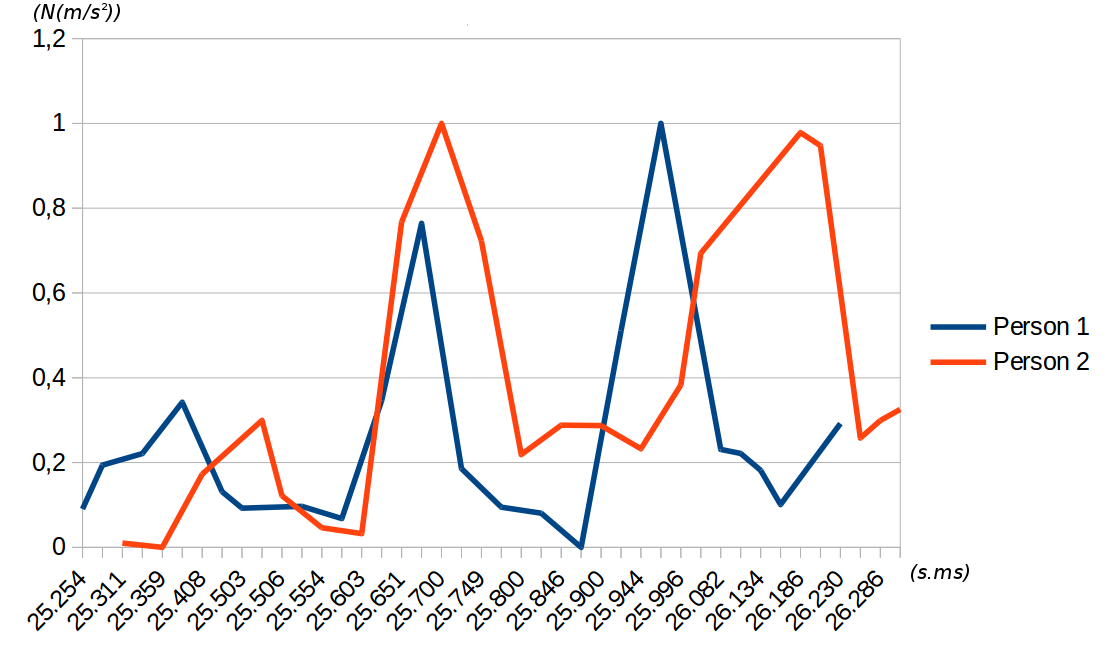
\includegraphics[scale=0.25]{Images/TwoFallsComparative.png}
  \caption[Acceleration during FAW fall]{Acceleration comparison during FAW fall.}
  \label{fig:FAWcomparison}
\end{figure}

For the FAW, we have decided to define the acceleration behaviour with normalised values; so the 
normalised acceleration behaviour during the FAW consists on:
\begin{enumerate}
 \item the variation of its values while the person is walking. We have divided this rule in two rules:
 \begin{enumerate}
  \item The normalised acceleration values go increasing in a range [0, 0.35].
  \item The normalised acceleration values go decreasing in a range [0, 0.35].
 \end{enumerate}
 \item as a consequence of the impact of the person against a wall, the acceleration normalised value 
 has to be greater than 0.7.
 \item the normalised acceleration values decreases to a range [0, 0.35]. The values of the acceleration are 
 in the mentioned range depending on the size of the person; the larger person results in a longer range 
 and if the person retains a position prior to a fall thanks to the wall. Moreover, a subtle peak could 
 appear as a consequence of a rebound.
 \item a second impact happens when the person hit the ground, the acceleration normalised values has to 
 be greater than 0.7.
 \item finally, the person is laying on the ground and the normalised acceleration value decreases. The 
 values of the acceleration are between [0.10, 0.35] and no subtle peaks appear. 
\end{enumerate}

The same analysis process has been done to the rest of sensors, and the behaviour of the acceleration of all of 
them follows the same pattern.

\subsubsection*{To define the fall event} Once the fall acceleration behaviour has been observed, the next step is to define the 
fall event in order to generate test events with IoT-TEG~\cite{TesisGutierrez2017,Gutierrez2017}. As it was explained in 
subsection~\ref{iotteg}, the event type attributes have
to be defined using the \texttt{<field>} element. The fall event contains one attribute, the acceleration, which is float, 
\texttt{type=``Float''}, and its values are not quoted, \texttt{quotes=``false''}. A new parameter in IoT-TEG has been defined as a 
consequence of the previous falls study. Given that the acceleration values follow a specific behaviour, it is necessary to include 
the \texttt{custom\_behaviour} property in the \texttt{<field>} element to define the behaviour of any event attribute; 
in this study, the acceleration. In the \texttt{custom\_behaviour} property the path to the file that includes the behaviour of the 
event attribute has to be written. The Example~\ref{FallEvent} shows the complete fall event definition (FallEventType).

\begin{lstlisting}[basicstyle=\ttfamily\footnotesize,language=XML,caption={Fall event type definition},label=FallEvent]
<?xml version="1.0" encoding="UTF-8"?>
<event name="FallEventType">
<block name="feeds" repeat="100">
 <field name="acceleration" quotes="false" type="Float" 
 custom_behaviour="/Path/To/Rule/File"></field>
</block>
</event>
\end{lstlisting}

IoT-TEG includes a new functionality, which has been implemented to simulate the desired behaviour of an 
event attribute with a \texttt{custom\_behaviour} property in its event type definition. This functionality 
allows to generate values of the event attribute following a behaviour that the user has described in a file.
In order to explain how the user has to define the desired behaviour of an event attribute, we are going
to use the FAW fall behaviour rules (see Example~\ref{FAWFallRules}). In a XML file the number of simulations has to be
indicated, the events involved in a simulation will be calculated according to the total number of events
to generate and the desired simulations. For example, if the number of test events to generate is 100, 
number indicated in the event type definition file, \texttt{repeat="100"}, and the number of desired 
simulations is 5, \texttt{simulations="5"}, number indicated in the behaviour rules definition file, 
the number of events involved to simulate the behaviour is 20. In the FAW fall example, the user ask to 
generate 100 test events and 5 falls (simulations), so 20 events will be used to define a FAW fall.

Variables can be defined if they are needed in the behaviour rules. They can be defined in the file where
the behaviour rules are included using the \texttt{<variables>} tags. To define them a name and a value 
have to be given to the variables. The value can be defined as a fixed value with the \texttt{value} 
property, or using a range with the \texttt{min} and \texttt{max} properties. Moreover, in some variables
are involved in the value of another variables; this is indicated using the variable with an specific 
format \texttt{\$(variable)}, see Example~\ref{FAWFallRules}. In addition, arithmetic operations can be 
done in the definition of the variable values. Let us see how using them in the FAW fall example. To 
define the acceleration behaviour during a FAW fall three variables are defined: \texttt{Base}, 
\texttt{ImpactWall} and \texttt{Impact}. Given that the acceleration behaviour during a FAW fall has
being done according to the normalised values, the variables and rules have been defined according to 
that analysis. The acceleration value in a stationary position is variable depending on the person, so 
we have considered the established value, $1g\approx9.81m/s^{2}$. That is the fixed value of the 
\texttt{Base} variable. To determine the values of the impacts, we have taken into account that the 
normalised value have to be $> 0,7$. So, to ensure that the impacts, \texttt{ImpactWall} and 
\texttt{Impact}, have a value meeting the mentioned condition the minimum value of the impact is the 
sum of the \texttt{Base} and \texttt{Base} multiply by \texttt{Base}$*0,7$; and the maximum value of the
impacts is $3g\approx9,81*3=$\texttt{Base}$*3$.

Once the variables are defined, the rules have to be determined. The first step is to indicate the 
\texttt{weight} for each rule in order to calculate the number of events to generate for each rule for 
each simulation. Following the simulation values the number of events to generate for each rule, according 
to the assigned weights, is: $20 * 0,25 = 5$ events will be generated for the first rule, another 5 events 
for the second rule, 1 event for the third rule, 5 events for the fourth rule, 1 event for the fifth
rule and the remained events, three events, for the sixth rule. We have to assign zero to the weight
\texttt{weight="0"} to indicate how the remained events have to be generated.

To define the rules, \texttt{min}, \texttt{max} and \texttt{value} properties can be used as well as the arithmetic 
operations and the references to another variables. Moreover, the \texttt{sequence} property can be used to obtain
values lower or higher than the one generated previously. The \texttt{sequence} property values are \texttt{inc}, 
to increase the value, or \texttt{dec}, to decrease the value.

\begin{lstlisting}[basicstyle=\ttfamily\footnotesize,language=XML,caption={Rules to define a FAW fall},label=FAWFallRules]
  <?xml version="1.0" encoding="UTF-8"?>
  <custom_conditions simulations="5">
  <variables>
   <variable name="Base" value="9.81"/>
   <variable name="ImpactWall" min="$(Base)+$(Base)*0.7" 
    max="$(Base)*3"/>
   <variable name="Impact" min="$(Base)+$(Base)*0.7" 
    max="$(Base)*3"/>
  </variables>
  <rules>
   <rule weight="0.25" min="0" max="$(ImpactWall)*0.35" 
    sequence="inc"/>
   <rule weight="0.25" min="0" max="$(ImpactWall)*0.35" 
    sequence="dec"/>
   <rule weight="1" value="$(ImpactWall)"/>
   <rule weight="0.25" min="0" max="$(Impact)*0.35"/>
   <rule weight="1" value="$(Impact)"/>
   <rule weight="0" min="$(Base)+$(Base)*0.10"
    max="$(Impact)*0.35"/>
  </rules>
  </custom_conditions>
\end{lstlisting}

Thanks to the included properties and parameters in the IoT-TEG new functionality, the desired behaviour rules that
follow the normalised acceleration values can be defined. Given that we have considered to define the FAW fall behaviour
rules according to the normalised values, the values to generate depend on the maximum value. Due to there are two 
values that can be the highest one, \texttt{ImpactWall} or \texttt{Impact}, the rules that depend on the maximum 
value contains the reference to the value, \texttt{ImpactWall} or \texttt{Impact}, according to the proximity
of the rule. For instance, the first and second FAW fall rules contain a reference to \texttt{ImpactWall}, the impact 
in the wall (third rule), which happens after the person is walking, something described in the first and the second rules.
The fourth and sixth rules contain a reference to \texttt{Impact}, the impact on the ground (fifth rule), which happen
after the person is falling and the person is laying on the floor, fourth and sixth rules.

It is needed to highlight that to obtain these rules to define the behaviour of the normalised acceleration several test
have been done. Once we obtained the desired results, test events were generated as they were necessary. The 
Figure~\ref{fig:IoTTEGFAWGeneratedEvents} shows the acceleration values of some of the generated FAW falls using
IoT-TEG and the new functionality.

\begin{figure}[!ht]
  \centering
  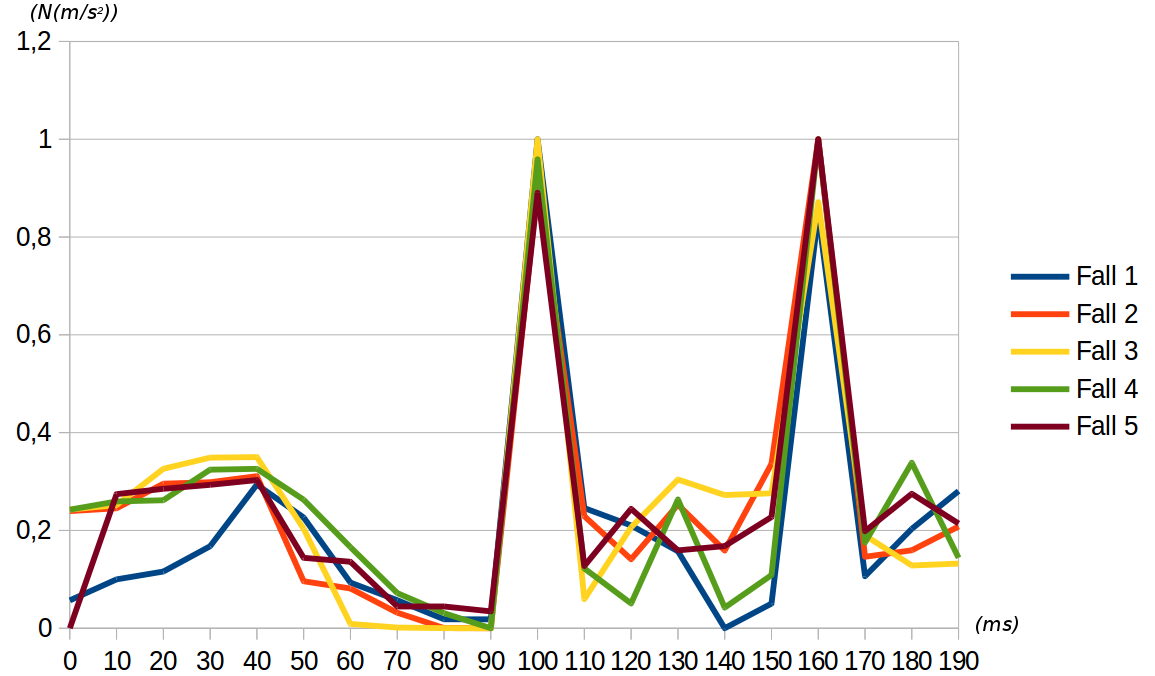
\includegraphics[scale=0.25]{Images/IoTTEGFAWGeneratedEvents}
  \caption[IoT-TEG generated FAW falls]{IoT-TEG generated FAW falls.}
  \label{fig:IoTTEGFAWGeneratedEvents}
\end{figure}

\subsection{Detected problems}
\label{sub:detectedproblems}

After testing the used fall detection prototype, some problems were 
found. Moreover, some considerations will be applied in future tests.

First of all, we are going to explain the problems related to the prototype; problems related to its hardware and
software. Talking about the software, the synchronisation in the prototype is an issue; we have founded the following problems:

\begin{itemize}
 \item In one hand, the falls from the beginning always should be discarded because the sensors are 
 sending a lot of data. The Table~\ref{tabla:Synchro} will be used to explain the problem. Let us say 
 that in ``fall 1'', there are more than 30 values that define the fall, and later in ``fall 3'', there are 
 12 values that define the fall. So, in order to analyse the falls and compare the acceleration behaviour, it is 
 difficult to work with that information. A comparison of two FAW falls with the synchronisation problem is shown
 in Figure~\ref{fig:synchronisation1}; the sensor 1 acceleration values for the first FAW fall are coloured in blue and the
 sensor 1 acceleration values for the second FAW fall are coloured in red. The first fall is one fall from the beginning
 of the simulation, and the second one is from the middle of the simulation.
 
 \begin{table}[!ht]
 \centering
 \begin{tabular}{*{5}{r}}
   \centering
\begin{tabularx}{9.5cm}{@{}ccc|ccc@{}}
  \toprule
  \multicolumn{1}{p{0.65cm}}{\centering \textsc{Time} \\ ($s.ms$)}  &  \multicolumn{1}{p{0.65cm}}{\centering \textsc{Accel.} \\ ($m/s^2$)}  &  \multicolumn{1}{p{2cm}}{\centering \textsc{N. Accel.} \\ ($N(m/s^2)$)}  &  \multicolumn{1}{p{0.65cm}}{\centering \textsc{Time} \\ ($s.ms$)}  &  \multicolumn{1}{p{0.65cm}}{\centering \textsc{Accel.} \\ ($m/s^2$)} &  \multicolumn{1}{p{2cm}}{\centering \textsc{N. Accel.} \\ ($N(m/s^2)$)} \\
  \midrule
25.561 & 9,81 & 0,11 & 25.546 & 8,73 & 0,1 \\
25.561 & 9,81 & 0,11 & 25.596 & 8,04 & 0,07 \\
25.562 & 11,38 & 0,17 & 25.645 & 13,93 & 0,35 \\
25.564 & 11,38 & 0,17 & 25.693 & 22,76 & 0,76 \\
25.609 & 15,11 & 0,33 & 25.742 & 10,59 & 0,19 \\
25.610 & 15,11 & 0,33 & 25.791 & 8,63 & 0,09 \\
25.610 & 15,11 & 0,33 & 25.841 & 8,34 & 0,08 \\
25.611 & 15,11 & 0,33 & 25.888 & 6,67 & 0 \\
25.612 & 31,4 & 1 & 25.937 & 17,46 & 0,51 \\
25.612 & 23,84 & 0,69 & 25.986 & 27,76 & 1 \\
25.657 & 23,84 & 0,69 & 26.082 & 11,58 & 0,23 \\
25.657 & 23,84 & 0,69 & 26.084 & 11,38 & 0,22 \\
25.658 & 23,84 & 0,69 &  &  & \\
25.659 & 23,84 & 0,69 &  &  & \\
25.660 & 9,52 & 0,10 &  &  & \\
25.660 & 9,52 & 0,10 &  &  & \\
25.706 & 9,52 & 0,10 &  &  & \\
25.706 & 9,52 & 0,10 &  &  & \\
25.707 & 9,52 & 0,10 &  &  & \\
25.707 & 9,52 & 0,10 &  &  & \\
25.708 & 23,74 & 0,69 &  &  & \\
25.709 & 23,74 & 0,69 &  &  & \\
25.756 & 23,74 & 0,69 &  &  & \\
25.756 & 23,74 & 0,69 &  &  & \\
25.757 & 27,86 & 0,85 &  &  & \\
25.758 & 27,86 & 0,85 &  &  & \\
25.758 & 9,52 & 0,1 &  &  & \\
25.759 & 9,52 & 0,1 &  &  & \\
25.760 & 9,52 & 0,1 &  &  & \\
25.804 & 7,06 & 0 &  &  & \\
25.805 & 7,06 & 0 &  &  & \\
25.805 & 7,06 & 0 &  &  & \\
25.806 & 7,06 & 0 &  &  & \\
  \bottomrule
\end{tabularx}

 \end{tabular}
 \caption{Synchronisation problem, fall 1 and fall 2}%
 \label{tabla:Synchro}
 \end{table}
 
 \begin{figure}[!ht]
  \centering
  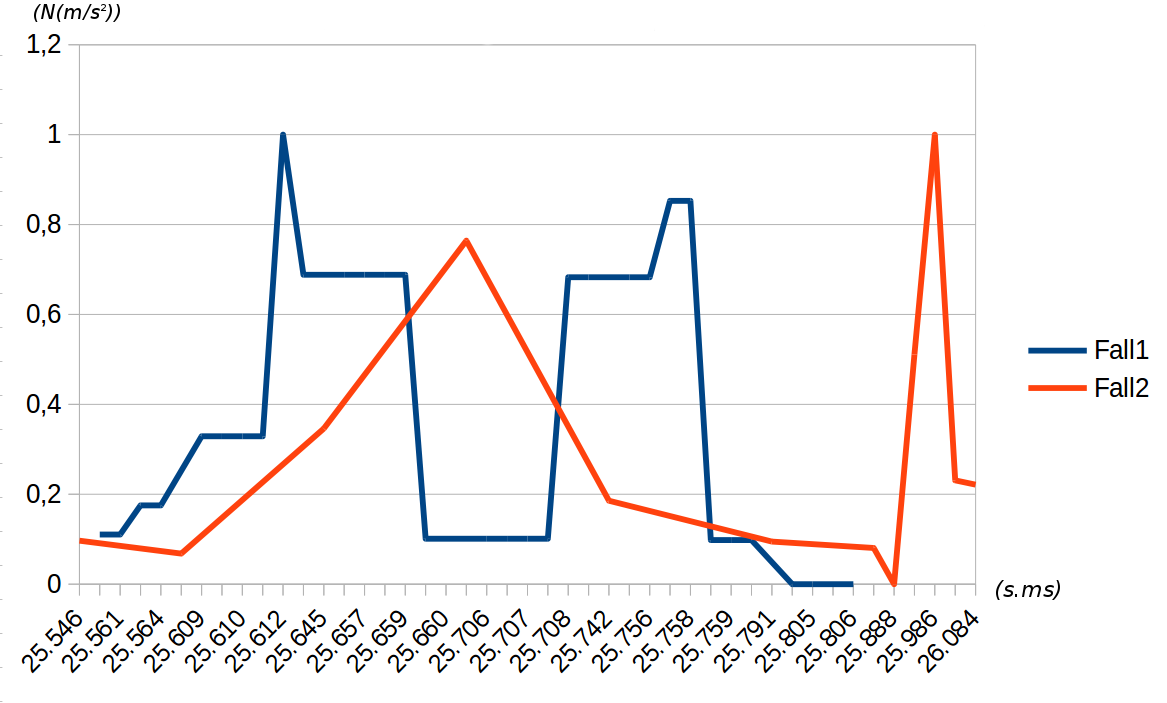
\includegraphics[scale=0.24]{Images/synchronisation1.png}
  \caption[Comparison acceleration during two FAW falls]{Synchronisation problem; comparison of acceleration values during two FAW falls.}
  \label{fig:synchronisation1}
 \end{figure}
 
 The acceleration values show that in less than 250 milliseconds there are more than 30 values from ``fall 1'', and
 in more than 350 milliseconds there are 12 values from ``fall 2''. There is a lack of synchronisation not only in
 the amount of data, but also in the time.
 
 \item On the other hand, some sensors transmit more data than the others; no matter the fall, the sensors are not 
 sending the same amount of data, even sometimes there is no data. The four sensors were working while the FAW fall
 simulation, but the obtained acceleration values were from three of them, one of the sensor does not transmit data 
 in one moment of the simulation, see Figure~\ref{fig:synchronisation2}.
 
 \begin{figure}[!ht]
  \centering
  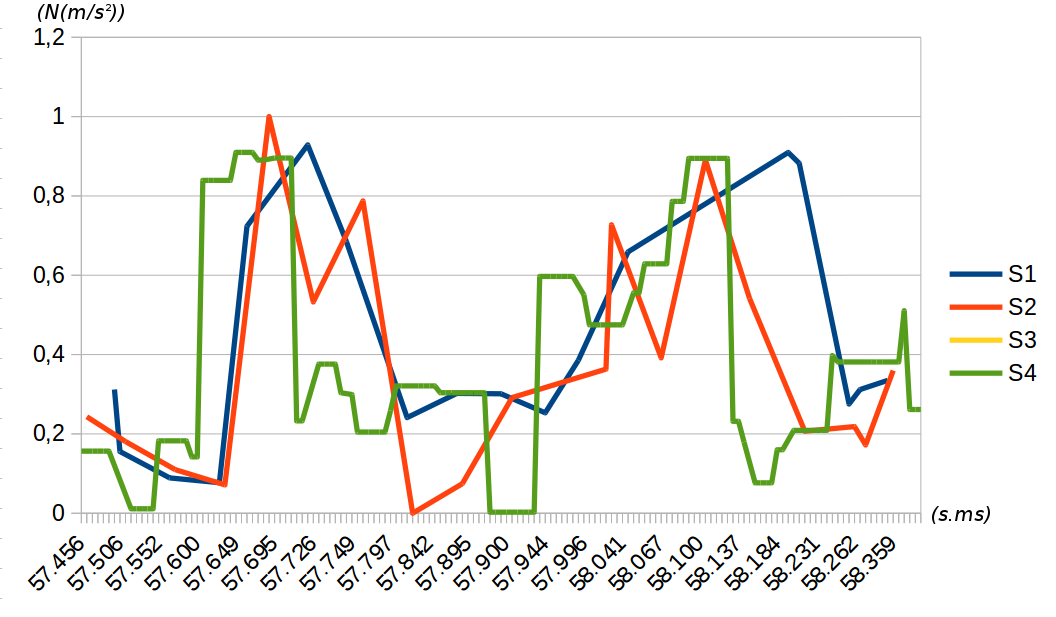
\includegraphics[scale=0.25]{Images/synchronisation2.png}
  \caption[Comparison acceleration during two FAW falls]{Synchronisation problem; acceleration values from the four sensors during a FAW fall.}
  \label{fig:synchronisation2}
 \end{figure}
\end{itemize}

\section{Example application of STAMP as hazard analysis method}
\label{sec:STAMP}

\subsection{Introducing STAMP}
A fall-detection system is a safety critical system requiring certification according to a safety standard (e.g. IEC 60601-1) \cite{international2005medical}. To satisfy functional safety requirements it is fundamental to apply hazard analysis methods during all development phases and operation to analyze the behavior of the system in case of malfunctioning. This technique should be applied already in the early design phases to counteract developmental errors \cite{STAMPThesis}. In the following STAMP will be applied in some architectural parts of the fall-detection system for functional safety validation.

STAMP (System-Theoretic Accident Model and Processes) is a comprehensive hazard analysis method based on system theory. A major goal of this approach is to control or eliminate hazards. This approach proposed by Leveson \cite{leveson2011engineering} is used to identify probable accident causes that are categorized as follows:
\begin{itemize}
	\item Accidents based on hardware and software component failure
	\item Unsafe interactions among components
	\item Complex human machine interfaces and human error models
	\item Erros in system design
	\item Faulty requirements
\end{itemize}  
STAMP treats accidents as a control problem. To prevent accidents safety constraints derived from system safety requirements must be enforced inside the different system hierarchy levels. If the given safety constraints are violated accidents may occur. Checking the enforcement of safety constraints leads to an additional layer of system testing. 

\subsection{STAMP - Hazard analysis}
STAMP begins on the system level and proceeds top down into the system hierarchy. To apply STAMP the following steps must be followed:
\begin{itemize}
	\item \textbf{Definition of accidents:} Person has fallen and the fall was not detected by the system.
	\item \textbf{Definition of hazards:} Data from 1 to 5 sensors of the belt are not sufficiently correlated in time (synchronization error).
	\item \textbf{Definition of safety requirements \& constraints:} The safety requirements and constraints are based on the hazard which causes the accident. Safety constraints are used to describe non-permissible system operations to ensure a safe operating condition. A top level safety requirement is the real-time detection of fall-events. The timestamps of all four nodes must be synchronized. If constraints are violated system migrates to unsafe or hazardous state.
	\item \textbf{Definition of safety control structure:}
	A high-level safety control structure should be defined which contains the system's components and the process which should be controlled.The control structure below (see Figure. \ref{fig:STAMPLevel1}) depicts the control loop of the controlled process, the movement of the person.
	The sensors provide sensor data to the controller (smartphone). The smartphone contains a data acquisition algorithm to collect the incoming data and a fall-detection algorithm to analyze this data. If the event corresponds to a fall, the alert system on the mobile device will call the emergency services for intervention. The actuator part of the system contains the control of the data acquisition process, i.e. timers, sleep mode etc.
	\begin{figure}[!ht]
		\centering
<<<<<<< Updated upstream
		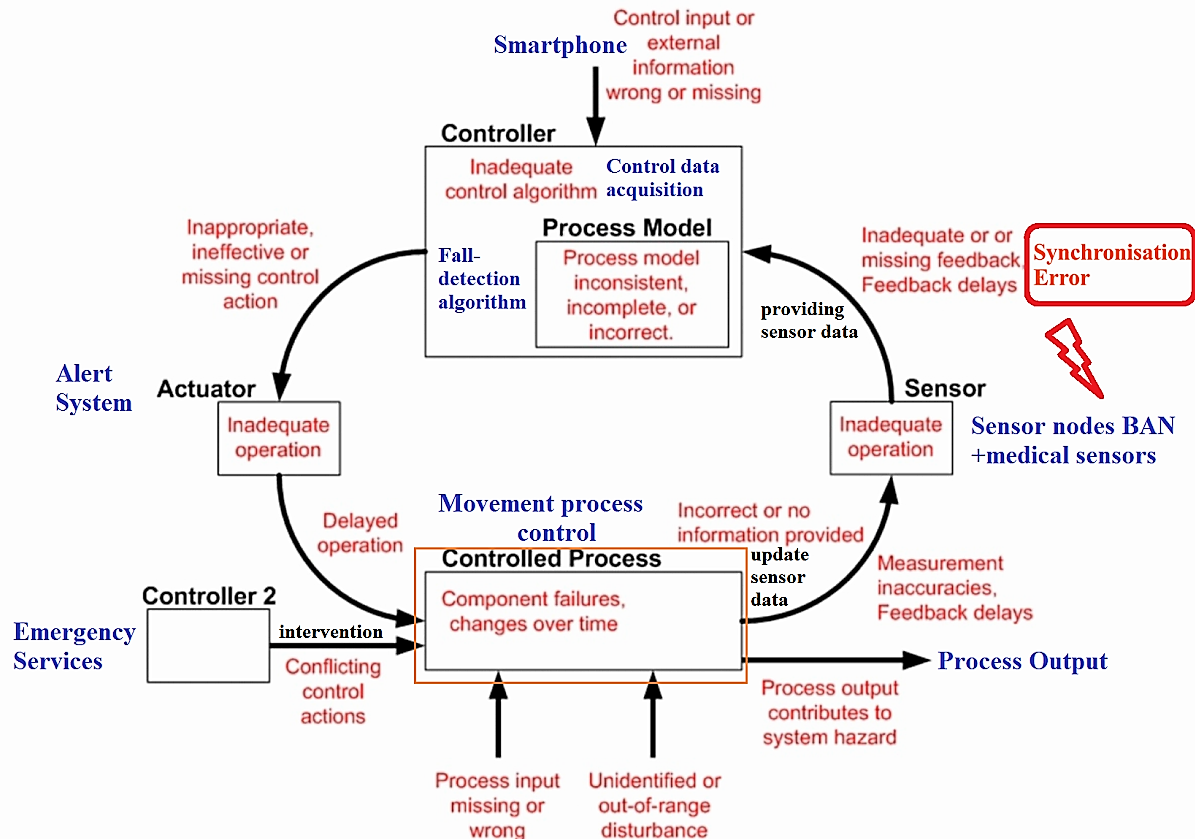
\includegraphics[scale=0.35]{Images/STAMP-SynchError}
		\caption[Safety Control Structure - Hierarchy level 2 \& 3]{Safety Control Structure - Hierarchy level 2 \& 3}
=======
		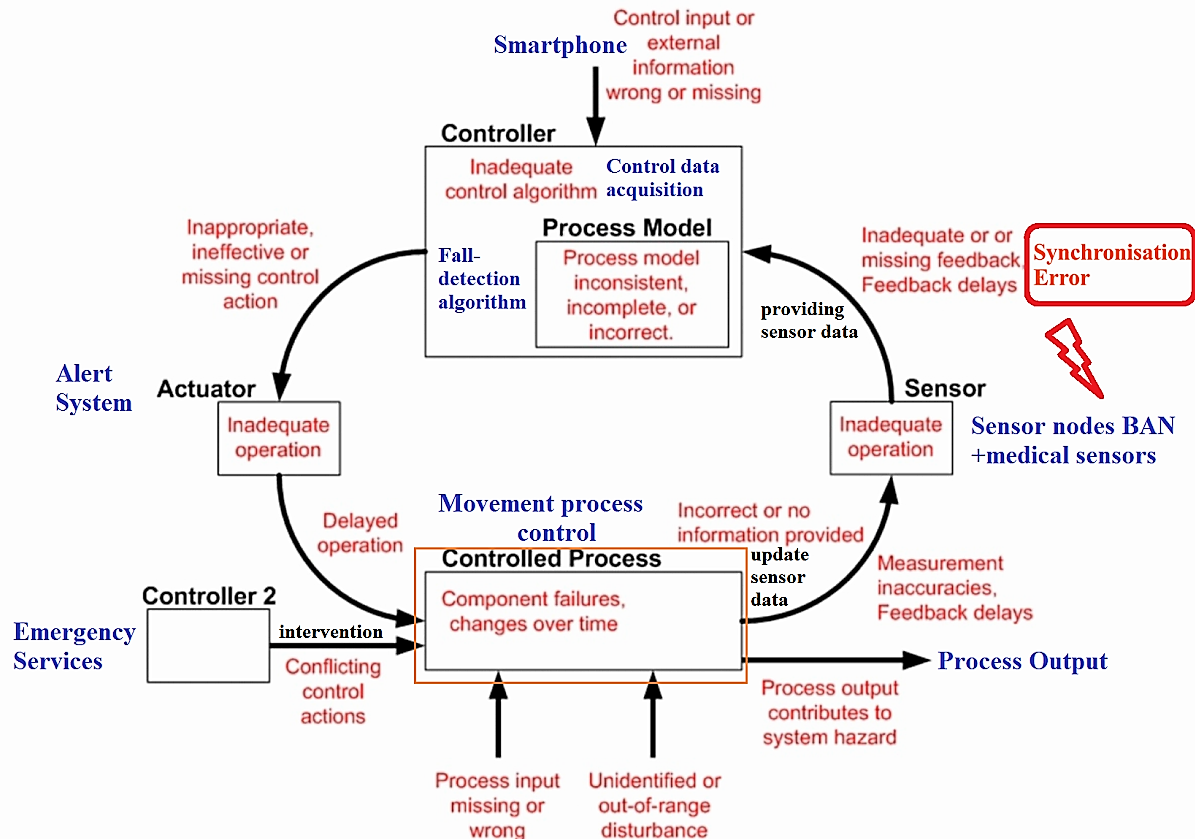
\includegraphics[scale=0.44]{images/STAMP-SynchError}
		\caption[System Safety Control Structure]{System Safety Control Structure - Hierarchy level 1) $\rightarrow$ Black label (system components), \textcolor{blue}{blue label (description of system components)}, \textcolor{red}{red label (possible hazards)}}
>>>>>>> Stashed changes
		\label{fig:STAMPLevel1}
	\end{figure}

	The lower level control loops (see Figure \ref{fig:STAMPLevel2+3}, \ref{fig:STAMPLevel4+5}) illustrate a detailed internal control structure of the controlled processes. These processes are interacting as a controller in the lower level structures. Taking into consideration the second level safety control loop, the movement process control (controller) receives the sensor data. Based on the data a control command will be executed to control the BAN which sends a feedback to the movement process controller. The third level control loop zooms into the BAN control, which is the master (controller) that actuates the wake up procedure of the sensor nodes to control the nodes. These will deliver sensor data, including the time to the BAN control.
	\begin{figure}[!ht]
		\centering
		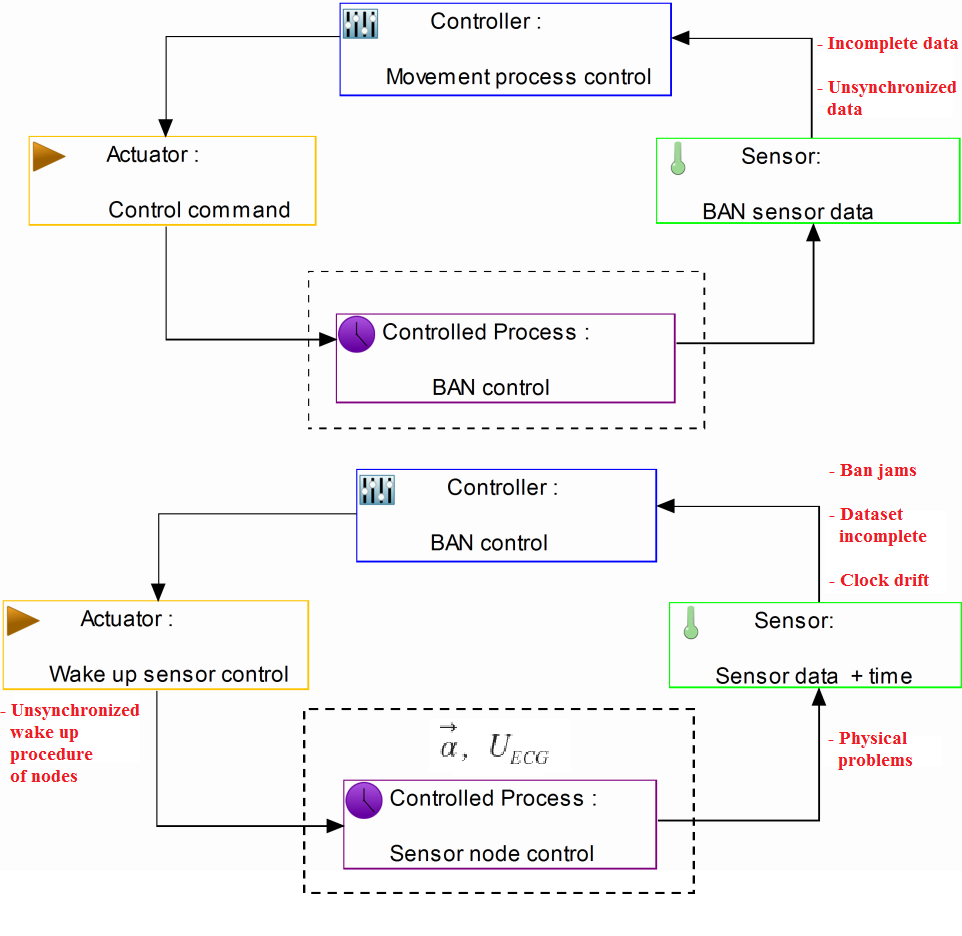
\includegraphics[scale=0.41]{Images/STAMP2+3level(2)}
		\caption[Safety Control Structure - Hierarchy level 2 \& 3]{Safety Control Structure - Hierarchy level 2 \& 3}
		\label{fig:STAMPLevel2+3}
	\end{figure}

 	To provide a more detailed hazard analysis two more control loop layers were created which are illustrated in the successive illustration (see Figure  \ref{fig:STAMPLevel4+5}). The fourth level of the system's control structure zooms into Sensor node control (controlled process, see Figure \ref{fig:STAMPLevel2+3}) which is the control unit (controller). Considering this control layer the controller receives the sensor's services and characteristics which are provided via Bluetooth Low Energy (BLE) and contain the sensor values. The sensor node control initiates a scanning command (actuator) to detect the sensor properties which are provided by the BLE - interface (controlled process: Bluetooth sensor detection control).  
	
		\begin{figure}[!ht]
		\centering
		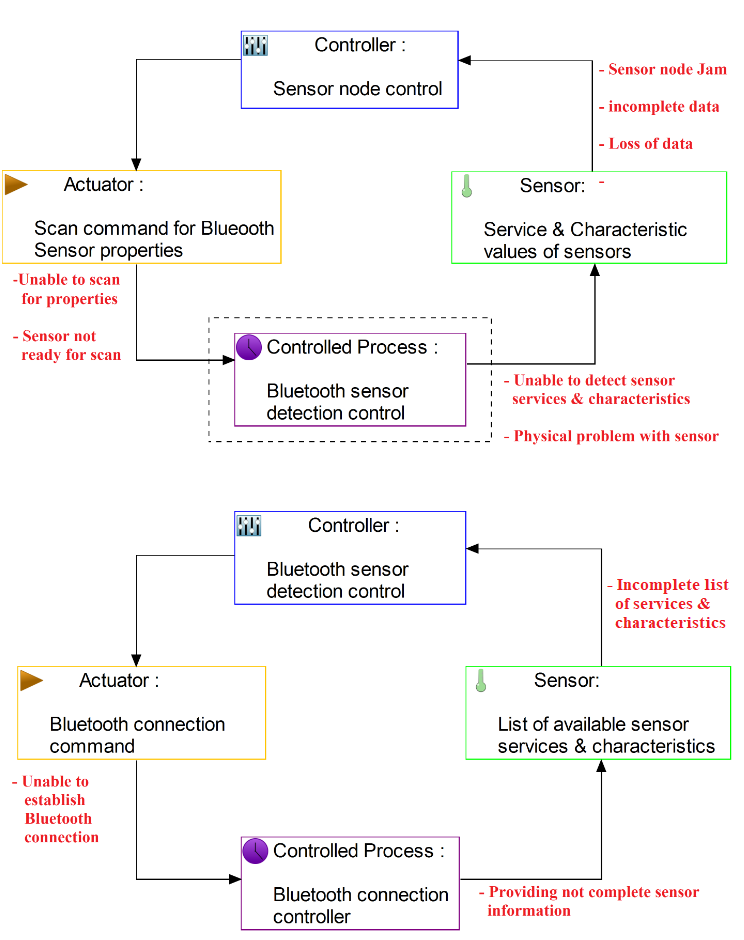
\includegraphics[scale=0.65]{Images/STAMP4+5level(2)}
		\caption[Safety Control Structure - Hierarchy level 4 \& 5]{Safety Control Structure - Hierarchy level 4 \& 5}
		\label{fig:STAMPLevel4+5}
	\end{figure}

	Taking into consideration the fifth level of the control loop which is depicted in figure \ref{fig:STAMPLevel4+5} an accurate view of the controlled process Bluetooth sensor detection control in level 4 is provided. The master Bluetooth sensor detection control (controller) actuates a connection command via BLE (actuator) to establish a connection to the sensors (controlled process: Bluetooth connection controller) which sends a list of available sensor's services and characteristics to the controller. 
	
	All these hazards (see red labels in Figure \ref{fig:STAMPLevel1}, \ref{fig:STAMPLevel2+3}, \ref{fig:STAMPLevel4+5}) lead to safety constraints. The incomplete list of sensor's services and characteristics (control loop - lower level 5) and sensor node jam (control loop - lower level 4) can lead to clock drift (control loop - lower level 3) and unsynchronized data (control loop - lower level 2) in the upper levels. Merging all the hazards from the lower levels may cause the synchronization error in the top level control structure and lead to violation of the safety constraint $\Delta$t $<=$ 50ms between the timestamps of the sensor nodes. The combination of these possible hazards makes the system inoperable to detect falls in real-time.
	

\end{itemize}


\section{Conclusion}
\label{sec:conclusion}
This work presents a wearable solution for fall detection that enhances the benefits of smart cities in terms of e-health. The tests performed with the test persons provided positive feedback regarding the use of this solution and a high acceptance of the system in application with smart cities was achieved. These results also show that falls are still a general problem in our daily life, which are underestimated and can lead to serious injuries or even fatal consequences. 

The test measurements carried out with the additional ECG sensor were positive and confirmed the approach of Gjoresk et al. \cite{Gjoreski2014} which allows a more accurate fall detection and, if necessary, a fall prediction. In the further development process it is planned to use machine learning or Complex Event Processing (CEP) in order to use certain ECG patterns in combination with the acceleration data. These should enhance a reliable detection of falls.

However, first the synchronization problem of the BAN must be solved, which can compromise the system's functionality. In order to solve this problem, a new hardware platform should be used, which contains a real time operating system, which facilitates the synchronization of different tasks in a wireless sensor network. In addition, the new microcontroller should also meet the requirements of patient compliance (see subsection \ref{subsec:Architecture}).



\section*{Acknowledgment}
We would like to thank the test subjects for the time they spent testing the fall detection prototype. The feedback and test results are very valuable for the further development of the detection system. We would particularly like to thank Dr. Nicolette Fritsch-Wagner for her assistance during the validation of our ECG sensor and for explaining how important the use of medical sensors (ECG sensors) can be for the detection of falls. The information obtained is of great importance and is necessary for the efficient development of reliable fall detection solution. 

This research did not receive any specific grant from funding agencies in the public, commercial, or not-for-profit sectors.


\section*{References}

\bibliography{mybibfile}

\end{document}
